%%% dna_struct.tex --- 


\section{Background}
\label{sec:dna_struct-intro}

From a biological perspective it seems obvious that DNA is something else than random mix of A, T, G and C nucleotides. Genomes are composed of functional elements as can be protein-coding genes, or promoters but also by non-functional elements like repetitive elements that by definition can not be random when taken together. However to what extent can we state that genomes are not a random soup of 4 letters? From the first analysis of the human genome \cite{Lander2001} we have some idea of the proportion of each of the \textit{families} of elements \fref{fig:prop_rep}{}. Intuitively we could assume that the structure of DNA is different in those families of genomic elements (GE). The sequence of a protein-coding gene would represent a specific selection of nucleotides with surely the highest informational content, while introns would tend more to random assembly and finally we can easily imagine that simple repeats present some biases towards 2 or 3 nucleotides (e.g.: CpG islands).

\begin{figure}[htpb] 
\centering 
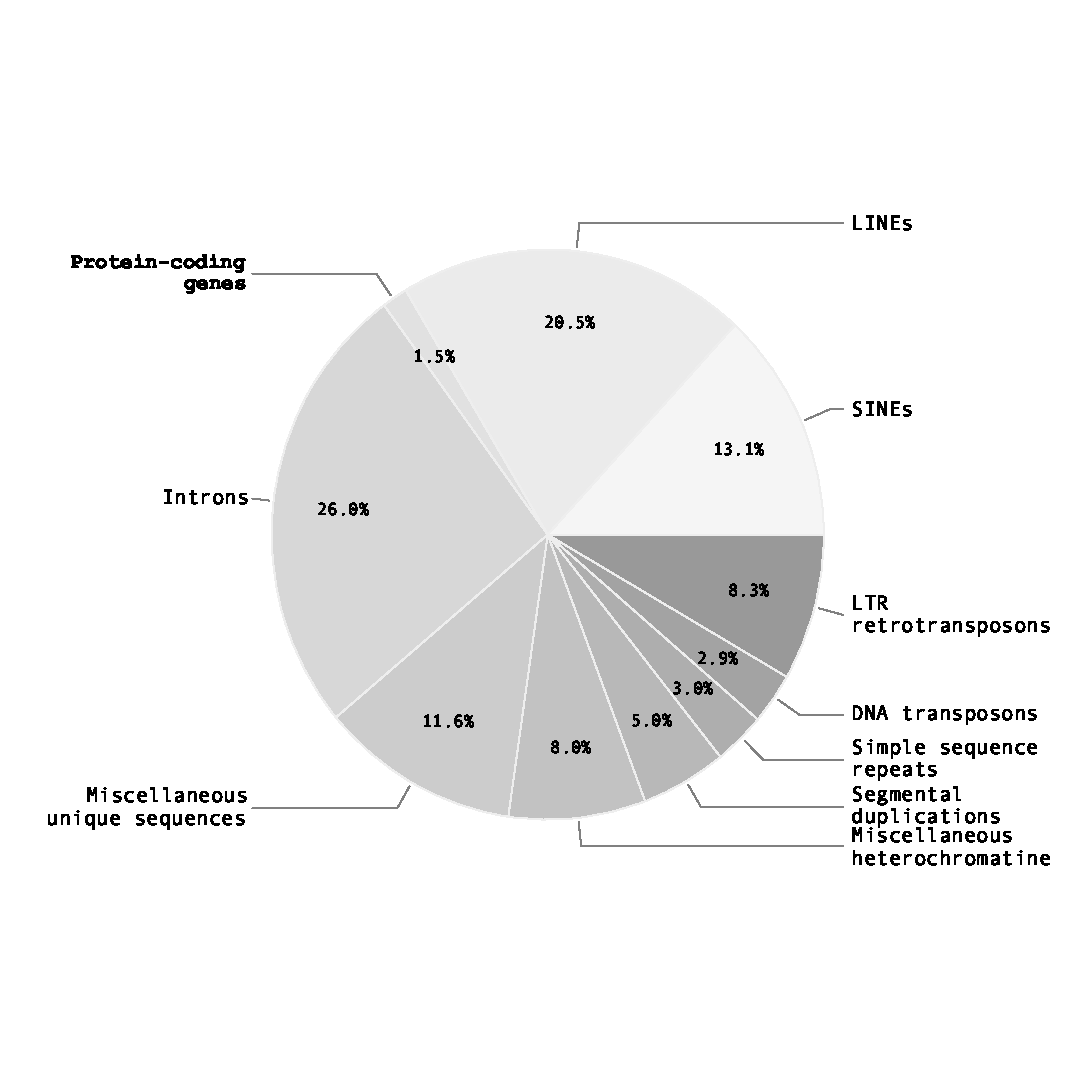
\includegraphics[trim=0cm 3cm 0cm 3cm, width=\textwidth]{tex_source/figures/dna_struct/prop_rep.pdf}
\caption[Genomic components of human genome]{{\bf Genomic components of human genome.}\\
Proportion of the major families of different genomic elements (GE) in the human genome according to \cite{Lander2001}}
\label{fig:prop_rep}
\end{figure}



\cite{Gregory2005}

This question could be solved in some sense by measuring genomes entropy. This measure presents the disadvantage that extreme cases of high entropy could correspond to \begin{inparaenum}[\itshape a\upshape)] \item {\bf a specially high content of information}, entropy-based algorithms are actually used to predict or confirm automatic detection of genes \cite{Du2006,Gerstein2007}, \item {\bf an exact random structure}, some work in the sense of testing the random structure of DNA have been done using entropy \cite{Loewenstern1999}. \end{inparaenum} However this characteristic of entropy could be only a semantic problem if we use it as a measure of relative variation in DNA complexity in genomes, and try to discern statistical patterns in the DNA sequences of different genomic element such as interspersed repeats or functional element (like protein-coding genes). This kind of description of 1DNA sequence complexity was already done by \cite{Holste2001}, but only in human chromosome 22.

\section{Results and Discussion}
\label{sec:dna_struct-result}

\subsection{Computing genome complexity}
\label{sec:comp-genome-compl}


Complexity value (CV) of complete genomes of 54 species of 20 major systematic groups of organisms, ranging 3.4Gb to 1.6Kb genome size was computed \tref{tab:genome}. The distribution of these complexity values showed an accurate fit to a linear regression model when genome size was used as the independent variable, with p $<$ 2.0e-16, \fref{fig:gen_compl}{-A}. The slope (alpha) of the regression (alpha=0.967), was very close to the maximum complexity slope (alpha = 1). Residual variation around the fitted regression was almost null (adjusted-R2 = 0.987). The fit of genomes to almost maximum complexity slope is remarkable considering that the linear model covers six order of magnitude of genome size along all diversity of life. From the shortest single-strand RNA genome of \textit{Hepatitis D} virus (size $\sim$ 1.69e+03 bp) to the largest double-strand DNA genome of the short-tailed opossum (size $\sim$ 3.41e+09 bp). Obligate endosymbionts bacteria with extreme reduction of genome size (\textit{Carsonella ruddii}, \textit{Buchnera aphidicola}, and \textit{Ureaplasma urealyticum}) \cite{Wernegreen2002}; parthenogenetic crustaceans with ubiquitous duplications of genes (\textit{Daphnia pulex}), archean organisms living in extreme environmental conditions (\textit{Sulfolobus islandicus}, \textit{Methanocaldococcus vulcanius}, \textit{Thermococcus sibiricus}), eukaryotes with a variable number of repetitive families, as well as the first synthetic organism made by humans (\textit{Synthetic mycoplasma mycoides}) \cite{Gibson2010}, fit the slope of the linear regression model. 

\begin{FPtable}
\raggedright
\resizebox{418pt}{!}{%
  \begin{tabular}{ l l p{62pt} l r r r r }
  \hline
  \textbf{Features} & \textbf{Species} & \textbf{ACN-EV} &
  \textbf{Clade} & \multicolumn{1}{l}{\textbf{GS}} &
  \multicolumn{1}{l}{\textbf{GC}} & \multicolumn{1}{l}{\textbf{GCR}} &
  \multicolumn{1}{l}{\textbf{Dmax}} \\ \hline
RNA & Hepatitis B & NC3977.1 & Virus & 1,682 & 1,671 & 1 & 0 \\
SGS-RNA & Hepatitis D & D01075.1 & Virus & 3,215 & 3,210 & 0.9984 & 0.0016 \\
SSD & Tomato mosaic & NC010836 \& NC10835.1 & Virus & 5,058 & 5,040 & 0.9964 & 0.0036 \\
SSD & Enterobacteria phage m13 & V00604 & Phage & 6,407 & 6,367 & 0.9938 & 0.0062 \\
RNA & HIV 1 & NC001802 & Virus & 9,181 & 9,105 & 0.9917 & 0.0083 \\
RNA & Sudan ebolavirus & NC006432 & Virus & 18,875 & 18,842 & 0.9983 & 0.0017 \\
DSD & Enterobacteria phage lambda & NC001416 & Phage & 48,502 & 48,381 & 0.9975 & 0.0025 \\
DSD & Human herpesvirus1 & NC001806 & Virus & 152,261 & 150,036 & 0.9854 & 0.0146 \\
SBG-IP-RG & Carsonella ruddii & NC008512  & Bacteria & 159,662 & 146,930 & 0.9203 & 0.0797 \\
IP-RG & Buchnera aphidicola & AE013218.1 & Bacteria & 642,122 & 626,533 & 0.9757 & 0.0243 \\
IP-RG & Ureaplasma urealyticum & CP001184 & Bacteria & 873,755 & 840,812 & 0.9623 & 0.0377 \\
SL & Synthetic mycoplasma mycoides & CP002027.1 & Bacteria & 1,078,809 & 1,026,444 & 0.9515 & 0.0485 \\
EE & Thermococcus sibiricus & CP001463.1 & Archaea & 1,242,891 & 1,237,320 & 0.9955 & 0.0045 \\
EE & Methanocaldococcus vulcanius & CP001787.1 & Archaea & 1,746,040 & 1,708,968 & 0.9788 & 0.0212 \\
EE & Sulfolobus islandicus & CP001731.1 & Archaea & 2,722,004 & 2,692,455 & 0.9891 & 0.0109 \\
 & Bacillus subtilis & {\it E!} Bacteria 9 & Bacteria & 4,215,606 & 4,198,057 & 0.9958 & 0.0042 \\
 & Mycobacterium tuberculosis & {\it E!} Bacteria 9 & Bacteria & 4,411,532 & 4,348,606 & 0.9857 & 0.0143 \\
 & Escherichia coli & CP001396.1 & Bacteria & 4,578,159 & 4,551,258 & 0.9941 & 0.0059 \\
LBG & Burkholderia xenovorans & NC007951-3 & Bacteria & 9,731,138 & 9,593,486 & 0.9859 & 0.0141 \\
AP & Saccharomyces cerevisiae & {\it E!} Fungi 3 & Fungi & 12,070,898 & 11,974,342 & 0.992 & 0.008 \\
UE & Plasmodium falciparum & {\it E!} Protists 9 & Apicomplexa & 23,263,332 & 21,070,640 & 0.9057 & 0.0943 \\
UE & Phaeodactylum tricornutum & {\it E!} Protists 9 & Heterokonta & 25,805,651 & 25,667,448 & 0.9946 & 0.0054 \\
UE & Dictyostelium discoideum & {\it E!} Protists 9 & Amebozoa & 31,199,234 & 31,023,020 & 0.9944 & 0.0056 \\
UE & Thalassiosira pseudonana & {\it E!} Protists 9 & Heterokonta & 33,919,934 & 30,877,496 & 0.9103 & 0.0897 \\
 & Ciona intestinalis & {\it E!} 62 & Urochordate & 87,649,861 & 84,674,396 & 0.9661 & 0.0339 \\
 & Caenorhabditis elegans & {\it E!} Metazoa 9 & Invertebrates & 100,272,217 & 97,720,472 & 0.9746 & 0.0254 \\
 & Tribolium castaneum & -1- & Invertebrates & 112,129,668 & 109,424,212 & 0.9759 & 0.0241 \\
AP-RG & Arabidopsis thaliana & {\it E!} Plants 9 & Plants & 118,960,082 & 116,563,556 & 0.9799 & 0.0201 \\
 & Drosophila melanogaster & {\it E!} Metazoa 9 & Invertebrates & 120,290,887 & 118,973,632 & 0.989 & 0.011 \\
GE & Daphnia pulex & {\it E!} Metazoa 9 & Invertebrates & 158,632,523 & 150,111,316 & 0.9463 & 0.0537 \\
AP & Arabidopsis lyrata & {\it E!} Plants 9 & Plants & 173,245,910 & 161,798,504 & 0.9339 & 0.0661 \\
AP & Tetraodon nigroviridis & {\it E!} 62 & Fishes & 208,708,313 & 207,067,712 & 0.9921 & 0.0079 \\
 & Apis mellifera & {\it E!} Metazoa 9 & Invertebrates & 224,750,524 & 219,278,732 & 0.9757 & 0.0243 \\
 & Anopheles gambiae & {\it E!} Metazoa 9 & Invertebrates & 225,028,531 & 221,180,624 & 0.9829 & 0.0171 \\
AP & Brachypodium distachyon & {\it E!} Plants 9 & Plants & 270,058,956 & 257,893,524 & 0.955 & 0.045 \\
AP & Oryza sativa & {\it E!} Plants 9 & Plants & 293,104,375 & 271,137,108 & 0.9251 & 0.0749 \\
AP & Populus trichocarpa & {\it E!} Plants 9 & Plants & 370,421,283 & 352,063,876 & 0.9504 & 0.0496 \\
AP & Physcomitrella patens & {\it E!} Plants 9 & Bryophyta & 453,927,385 & 399,508,556 & 0.8801 & 0.1199 \\
AP & Sorghum bicolor & {\it E!} Plants 9 & Plants & 625,636,188 & 491,993,216 & 0.7864 & 0.2136 \\
AP & Oryzias latipes & {\it E!} 62 & Fishes & 582,126,393 & 562,662,192 & 0.9666 & 0.0334 \\
 & Gallus gallus & {\it E!} 62 & Birds & 984,855,151 & 971,359,304 & 0.9863 & 0.0137 \\
 & Taeniopygia guttata & {\it E!} 62 & Birds & 1,013,982,659 & 996,918,996 & 0.9832 & 0.0168 \\
AP & Danio rerio & {\it E!} 62 & Fishes & 1,354,636,069 & 1,191,452,752 & 0.8795 & 0.1205 \\
AP-RP & Zea mays & {\it E!} Plants 9 & Plants & 2,045,697,632 & 1,197,255,904 & 0.5853 & 0.4147 \\
 & Canis familiaris & {\it E!} 62 & Mammals & 2,309,875,279 & 2,272,374,188 & 0.9838 & 0.0162 \\
 & Equus caballus & {\it E!} 62 & Mammals & 2,335,454,424 & 2,307,202,104 & 0.9879 & 0.0121 \\
 & Bos taurus & {\it E!} 62 & Mammals & 2,466,956,401 & 2,406,743,280 & 0.9756 & 0.0244 \\
 & Rattus norvegicus & {\it E!} 62 & Mammals & 2,477,053,718 & 2,430,894,052 & 0.9814 & 0.0186 \\
 & Mus musculus & {\it E!} 62 & Mammals & 2,558,509,481 & 2,521,038,616 & 0.9854 & 0.0146 \\
 & Pan troglodytes & {\it E!} 62 & Mammals & 2,598,733,311 & 2,566,544,200 & 0.9876 & 0.0124 \\
 & Macaca mulatta & {\it E!} 62 & Mammals & 2,646,263,164 & 2,621,196,144 & 0.9905 & 0.0095 \\
 & Pongo abelii & {\it E!} 62 & Mammals & 2,722,968,487 & 2,697,592,876 & 0.9907 & 0.0093 \\
 & Homo sapiens & {\it E!} 62 & Mammals & 2,858,658,095 &
 2,841,049,052 & 0.9938 & 0.0062 \\
LGS & Monodelphis domestica & {\it E!} 62 & Mammals & 3,412,593,369 & 3,402,944,248 & 0.9972 & 0.0028 \\ \hline
  \end{tabular}
}
\caption[Genomes Complexity.]%
{{\bf Genomes Complexity.} \\Genomes size (GS), genomes complexity (GC), genome complexity ratio ($GCR=\frac{GC}{GS}$), and deviation from the maximum GCR (Dmax=1-GCV) for 54 species of different taxa. NCBI accession number or Ensembl ({\it E!}) version (ACN-EV). {\bf \em Features}: {\bf AP}: Ancient Polyploid; {\bf DSD}: Double-Strand DNA; {\bf EE}: Extreme Environment; {\bf GE}: Gene Expansion; {\bf IP}: Intracellular Parasite; {\bf LBG}: Largest Bacterial Genome; {\bf LGS}: Largest Genome Sequenced; {\bf RG}: Reduced Genome; {\bf RNA}: RNA Virus; {\bf RP}: Recent Polyploid; {\bf SBG}: Shortest Bacterial Genome; {\bf SGS}: Shortest Genome Sequenced; {\bf SL}: Synthetic Life; {\bf SSD}: Single-Strand DNA; {\bf UE}: Unicellular Eukaryote. {\bf \em Notes}: -1-: \myurl{http://www.hgsc.bcm.tmc.edu/ftp-archive/Tcastaneum/Tcas3.0/}
}
\label{tab:genome}
\end{FPtable}


\begin{FPfigure}
\centering 
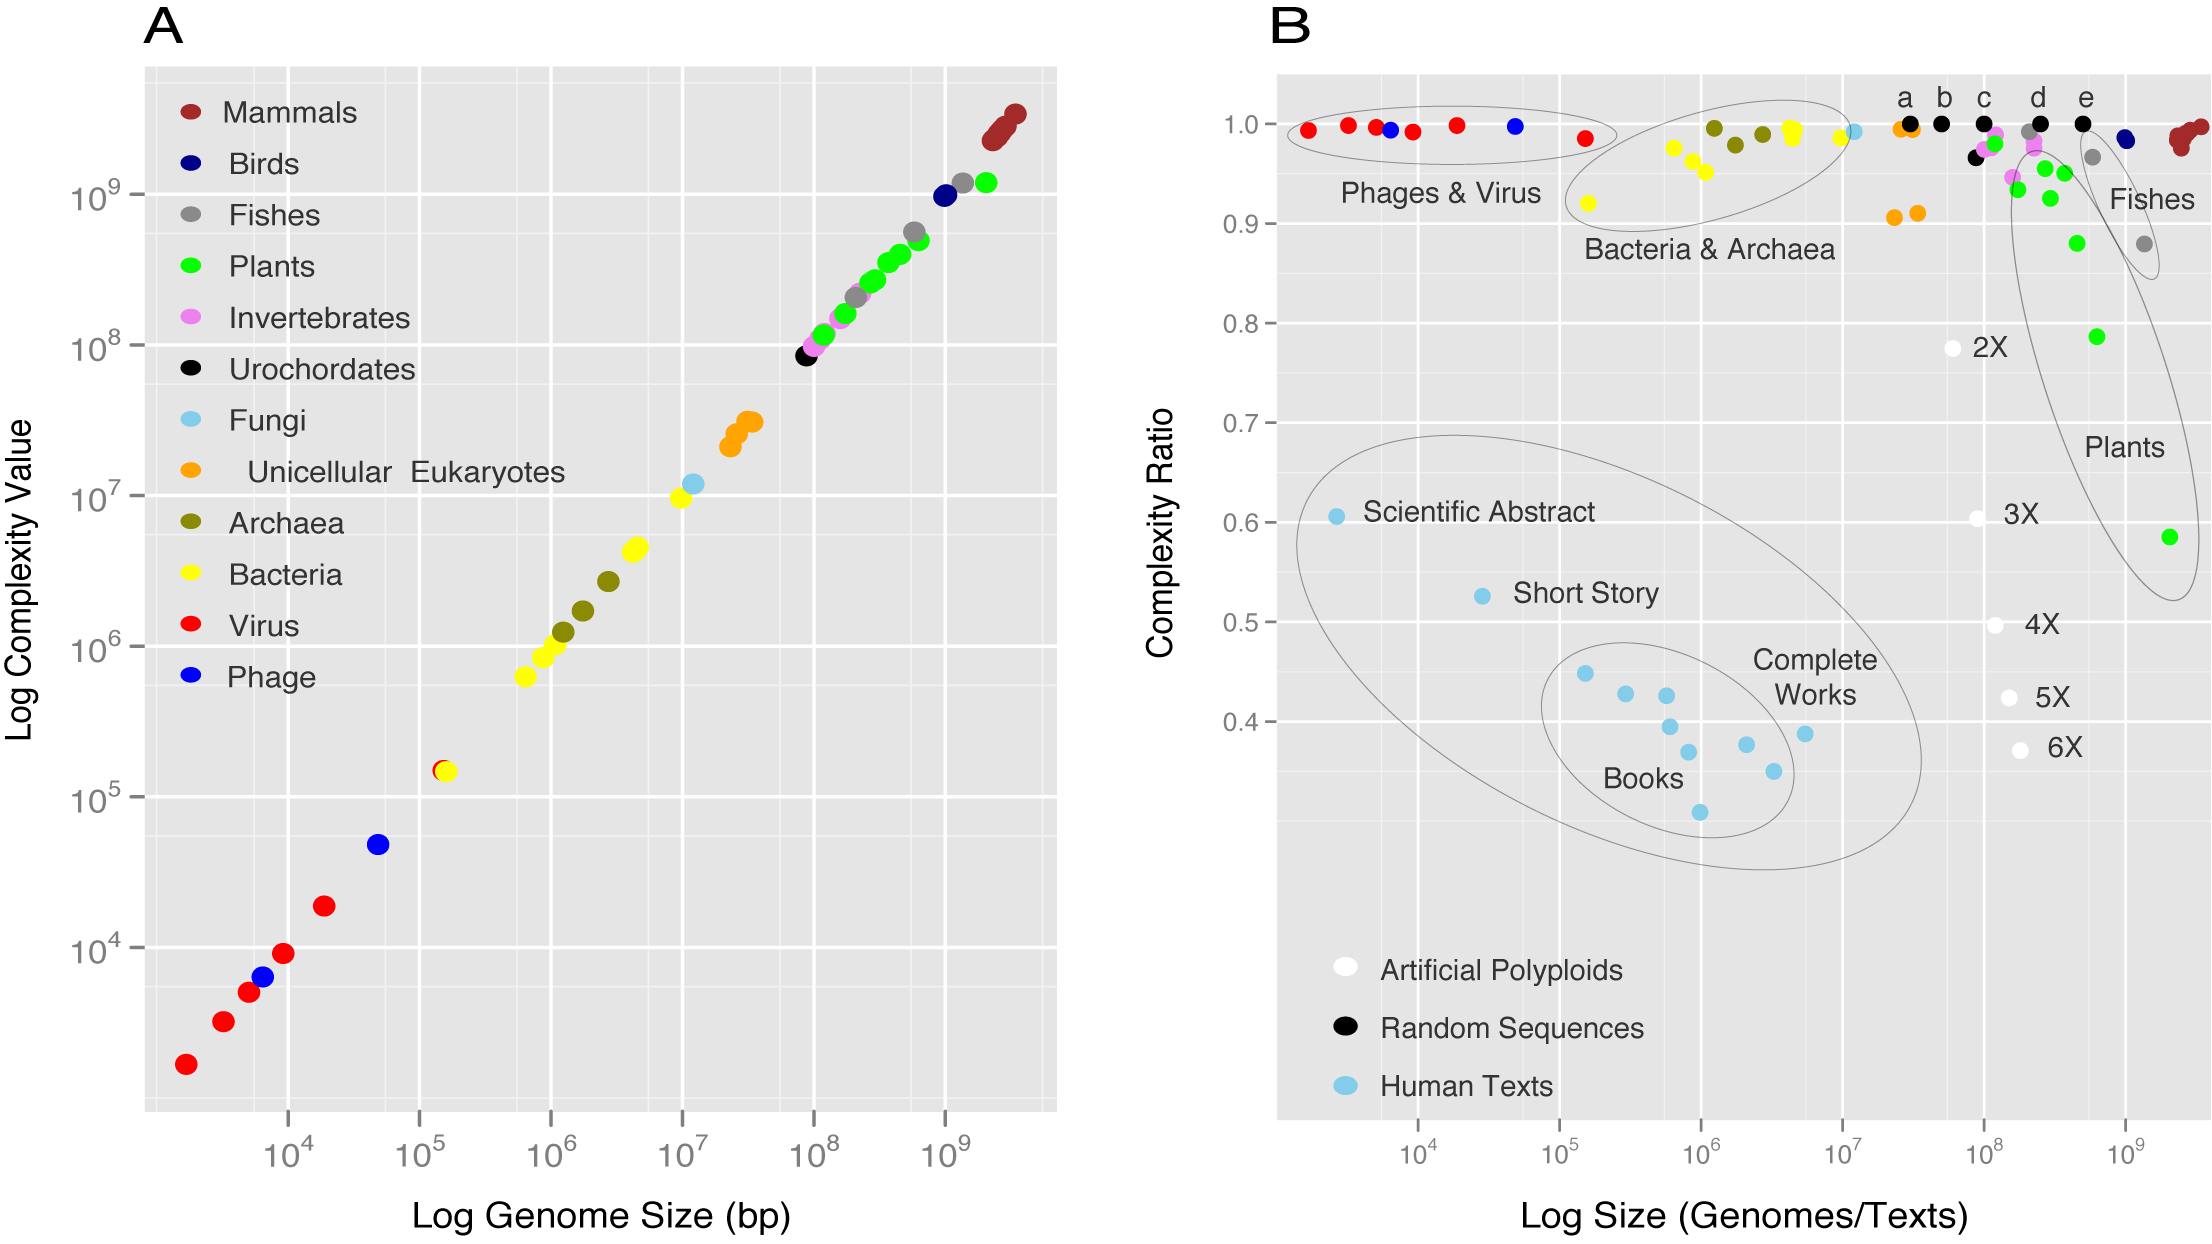
\includegraphics[width=\textwidth]{tex_source/figures/dna_struct/genome_complexity.png}
\caption[Genome complexity value]{{\bf Genome complexity value.} \\\textbf{(A)} Complexity values and genome size of 54 genomes. Log scales are used to display species diversity. Species listed by genome size increase are (see \tref{tab:genome} for details): \textit{Hepatitis D} (V), \textit{Hepatitis B} (V), \textit{Tomato mosaic} (V), \textit{Enterobacteria phage m13} (Ph), \textit{Hiv 1} (V), \textit{Sudan ebolavirus} (V), \textit{Enterobacteria phage lambda} (Ph), \textit{Human herpesvirus1} (V), \textit{Carsonella ruddii} (Ba), \textit{Buchnera aphidicola} (Ba), \textit{Ureaplasma urealyticum} (Ba), \textit{Synthetic mycoplasma mycoides} (Ba), \textit{Thermococcus sibiricus} (Ar), \textit{Methanocaldococcus vulcanius} (Ar), \textit{Sulfolobus islandicus} (Ar), \textit{Bacillus subtilis} (Ba), \textit{Mycobacterium tuberculosis} (Ba), \textit{Escherichia coli} (Ba), \textit{Burkholderia xenovorans} (Ba), \textit{Saccharomyces cerevisiae} (Fu), \textit{Plasmodium falciparum} (Ue), \textit{Phaeodactylum tricornutum} (Ue), \textit{Thalassiosira pseudonana} (Ue), \textit{Dictyostelium discoideum} (Ue), \textit{Ciona intestinalis} (Ur), \textit{Caenorhabditis elegans} (I), \textit{Tribolium castaneum} (I), \textit{Arabidopsis thaliana} (Pl), \textit{Drosophila melanogaster} (I), \textit{Daphnia pulex} (I), \textit{Arabidopsis lyrata} (Pl), \textit{Tetraodon nigroviridis} (Fi), \textit{Apis mellifera} (I), \textit{Anopheles gambiae} (I), \textit{Brachypodium distachyon} (Pl), \textit{Oryza sativa} (Pl), \textit{Populus trichocarpa} (Pl), \textit{Physcomitrella patens} (Pl), \textit{Oryzias latipes} (Fi), \textit{Sorghum bicolor} (Pl), \textit{Gallus gallus} (Bi), \textit{Taeniopygia guttata} (Bi), \textit{Danio rerio} (Fi), \textit{Zea mays} (Pl), \textit{Canis familiaris} (M), \textit{Equus caballus} (M), \textit{Bos taurus} (M), \textit{Rattus norvegicus} (M), \textit{Mus musculus} (M), \textit{Pan troglodytes} (M), \textit{Macaca mulatta} (M), \textit{Pongo abelii} (M), \textit{Homo sapiens} (M), \textit{Monodelphis domestica} (M). V: Virus, Ph: Phage, Ba: Bacteria, A: Archaea, Fu: Fungi, Ue: Unicellular eukaryote, Ur: Urochordate, I: Invertebrate, Pl: Plants, Fi: Fish, Bi: Bird, M: Mammal. \textbf{(B)} Most genomes have complexity ratio (CR) between 0.90 and 1.0. Four polyploid species have CR $<$ 0.9: P. patens (0.880), \textit{D. rerio} (0.879), \textit{S. bicolor} (0.786) and \textit{Z. mays} (0.585). a, b, c, d, e correspond to random [ACGT] strings of 30, 50, 100, 250 and 500 Mb length, respectively. 2$\times$ to 6$\times$ correspond to random polyploids [ACGT] sequences where 1$\times$ is ``a''. Changes in sequence length due to polyploidy produce no change in complexity ratio (see \tref{tab:book_compl}). Notice the low CR of human texts (see Table S3 for details). }
\label{fig:gen_compl}
\end{FPfigure}

We studied deviations of complexity value to the slope (alpha) by computing the complexity ratio (CR), and the deviation to the maximum ratio (Dmax = 1- CR). According to \tref{tab:genome}, only ten species showed Dmax $>$ 0.05. These are: six ancient or recent polyploid species; the most extreme case of genome reduction in bacteria; the explosive case of gene expansion in Daphnia, and two unicellular eukaryotes.

The highest CR=1 was obtained for non-polyploid (1$\times$), randomly generated sequences with uniform distribution of ACGT; however, CR falls exponentially when ploidy level increases reaching CR=0.25 for 10$\times$ \tref{tab:book_compl}. Differences in CR were calculated for polyploids after log transformation and linear regression model adjustment, providing a slope (alpha) = -0.81 (adjusted-R2 = 0.97, p $<<$ 0.0001). 

\begin{table}[htbp]
\resizebox{418pt}{!}{%
\begin{tabular}{ l l l r r r }
\hline
\textbf{Features} & \textbf{Author - Writings} & \textbf{Language} & \multicolumn{1}{l}{\textbf{L}} & \multicolumn{1}{l}{\textbf{C}} & \multicolumn{1}{l}{\textbf{CR}} \\ \hline
SA & C. Venter. The human genome (abstract) & English & 2,662 & 1,613 & 0.6059 \\
SS & J. L. Borges. El Aleph & Spanish & 28,507 & 14,991 & 0.5259 \\
B & A. Von Goethe. Torcuato Tasso & German & 152,104 & 68,187 & 0.4483 \\
B & H. Quiroga. Cuentos amor, locura y muerte & Spanish & 293,482 & 125,552 & 0.4278 \\
B & D. F. Sarmiento. Facundo & Spanish & 601,477 & 242,982 & 0.4259 \\
B & D. Alighieri. Divina Commedia & Italian & 570,480 & 301,609 & 0.3692 \\
B & I. Newton. Principia Mathematica & Latin & 817,032 & 237,558 & 0.395 \\
B & B C. Darwin. The Origin of species & English & 981,958 & 303,503 & 0.3091 \\
B & B M. Cervantes. El Quijote & Spanish & 2,097,943 & 790,702 & 0.3769 \\
B & B V. Hugo. Les Miserables & French & 3,259,269 & 1,141,378 & 0.3502 \\
CW & W. Shakespeare & English & 5,447,165 & 2,111,425 & 0.3876 \\ \hline
\end{tabular}
}
\caption[Human language Complexity]{\textbf{Human language Complexity}\\
Work length (L), complexity (C), complexity ratio (CR), and deviations from the maximum ratio of complexity (Dmax=1- CR) for 11 human writings in six different languages. Features: SA: Scientific abstract, SS: Short story; B: Book, CW: Complete Work
}
\label{tab:book_compl}
\end{table}

Complexity ratios of complete genomes, random sequences of different ploidy and human language texts are displayed in \fref{fig:gen_compl}{-B}. Maximum CR corresponds to random sequence of lengths ranging from 5 Kb to 2.5 Gb (a, b, c, d and e). Non-polyploid genomes showed CR $>$ 0.90. Within polyploids the lowest ratio corresponds to \textit{Z. mays} with CR=0.58, and the next to the lowest ratio, its closest relative \textit{S. bicolor} with CR=0.78. Overall strings analyzed, the lowest CR was obtained in human language texts. CR of 11 human texts of different sizes and languages, from short scientific abstract to the complete works of William Shakespeare, are also depicted \fref{fig:gen_compl}{-B} and \fref{fig:lang_compl}{}. CR diminishes as texts size increases, due to the limited lexicon and the fixed language grammar. Complexity reached the lowest ratio in Darwin's Origin of Species (~ 0.309), which is comparable to the CR of a random polyploid sequence of ~ 7$\times$. Observe that text sizes are contained in the range of phages, virus and bacteria genome sizes. Details of complexities of human writings are in shown \tref{tab:book_compl}.

\begin{figure}[htpb] 
\centering
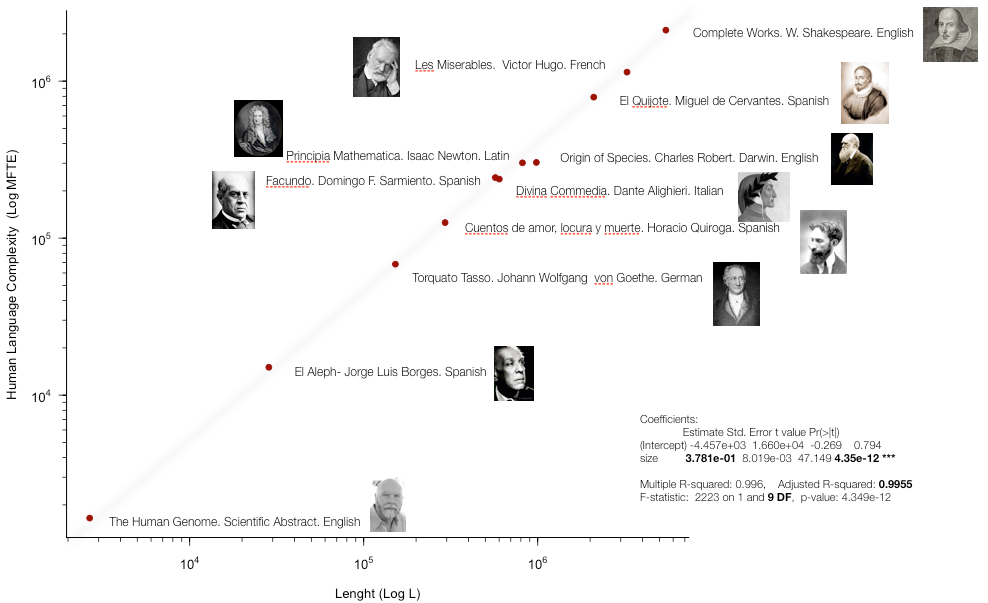
\includegraphics[width=\textwidth]{tex_source/figures/dna_struct/language_complexity.png}
\caption[Human language complexity]{{\bf Human language complexity.} \\
Complexity in human writings shows a constant increase with text length. Regression analysis shows that in contrast to genomes, human language is highly repetitive. While genomes match an almost perfect regression of slope ~1, human language complexity fits a linear regression model with slope alpha=0.378, (adjusted R = 0.995).}
\label{fig:lang_compl}
\end{figure}

\subsection{Genome complexity and ploidy level}
\label{sec:genome-compl-ploidy}

Recent polyploid species as maize and sorghum exhibited noticeably low complexity ratios, however, ancient polyploids and non-polyploids had indistinguishable complexity ratios. We tested the hypothesis that the observed genome complexity values are correlated with size and ploidy level. A categorical variable divided polyploid (ancient or recent), and non-polyploid species described in \tref{tab:genome}. The size-interaction term provided significant deviations (p $<$ 2e-16, adjusted-R2 = 0.997), while independent linear models slopes were 0.633 (p $<$ 4.8e-07, adjusted-R2 = 0.921), and 0.988 (p $<$ 2e-16, adjusted-R2 = 1.00) for polyploid and non-polyploid genomes. 

\subsection{Chromosome complexity}
\label{sec:chrom-compl}

Complexity value of each eukaryote chromosome (567 autosomes of 31 species) was computed and plotted against size \fref{fig:chr_compl}{-A}. Linear regression models considering the full dataset, or excluding polyploid species revealed a very significant statistical relationship (slope = 0.924, adjusted-R2 = 0.989, p $<$ 2e-16, or slope = 0.951, adjusted-R2 = 0.999, p $<$ 2e- 16, respectively). The adjustment of a linear regression model to chromosomes of polyploid species was statistically significant (p $<$ 2e-16, R2 = 0.982), while their complexity values exhibited a lower slope (alpha= 0.696), than the complexity values of chromosomes of non- polyploid species. Again, as was observed in genomes, the size-interaction term was statistically significant (p $<$ 2e-16), suggesting that complexity and size deviates differently for chromosomes of polyploid and non-polyploid species. Notice that for non-polyploid species the slope of their chromosome complexity values against size almost coincides with the slope of their genome complexity values (alpha = 0.989, 0.988, respectively). \fref{fig:chr_compl}{-B} displays CR for chromosomes. The boxplot inside shows the distribution of CR for all chromosomes. The fist quartile of the full sample indicates that 75\% of the data are above 0.958, while the median and mean was 0.974 and 0.964. The minimum CR value corresponds to maize chromosome 10 (0.683), and maximum to \textit{P. tricornutum} chromosome 28 (0.999). Opossum chromosome 1 (the largest chromosome) has a CR of 0.942. Mean CR of maize's chromosomes was 0.698, while maize genome CR was 0.585. The difference suggests extensive duplicated regions in maize chromosomes, which was previously described in \cite{Weber1989,Gaut2001} and attributed to a tetraploid event occurred in the origin of maize 11.4 My ago \cite{Gaut1997,Wolfe2001}. However, differences between mean chromosome to genome CR were observed in different species with variable deviations: sorghum (0.854:0.786), zebrafish (0.924:0.879), \textit{A. lyrata} (0.966:0.934), \textit{P. trichocarpa} (0.971:0.950), \textit{S. cerevisae} (0.996:0.992), and \textit{A. thaliana} (0.986:0.980), \textit{M. domestica} (0.944:0.997), \textit{M. musculus} (0.959: 0.985), and \textit{H. sapiens} (0.960:0.993). Appendix \ref{cha:repe-summ-outp} gives the values for the full data set. Further insights on chromosome and genome CR differences are discussed in the section on polyploid and return to maximum complexity, below.

\begin{figure}[htpb] 
\centering 
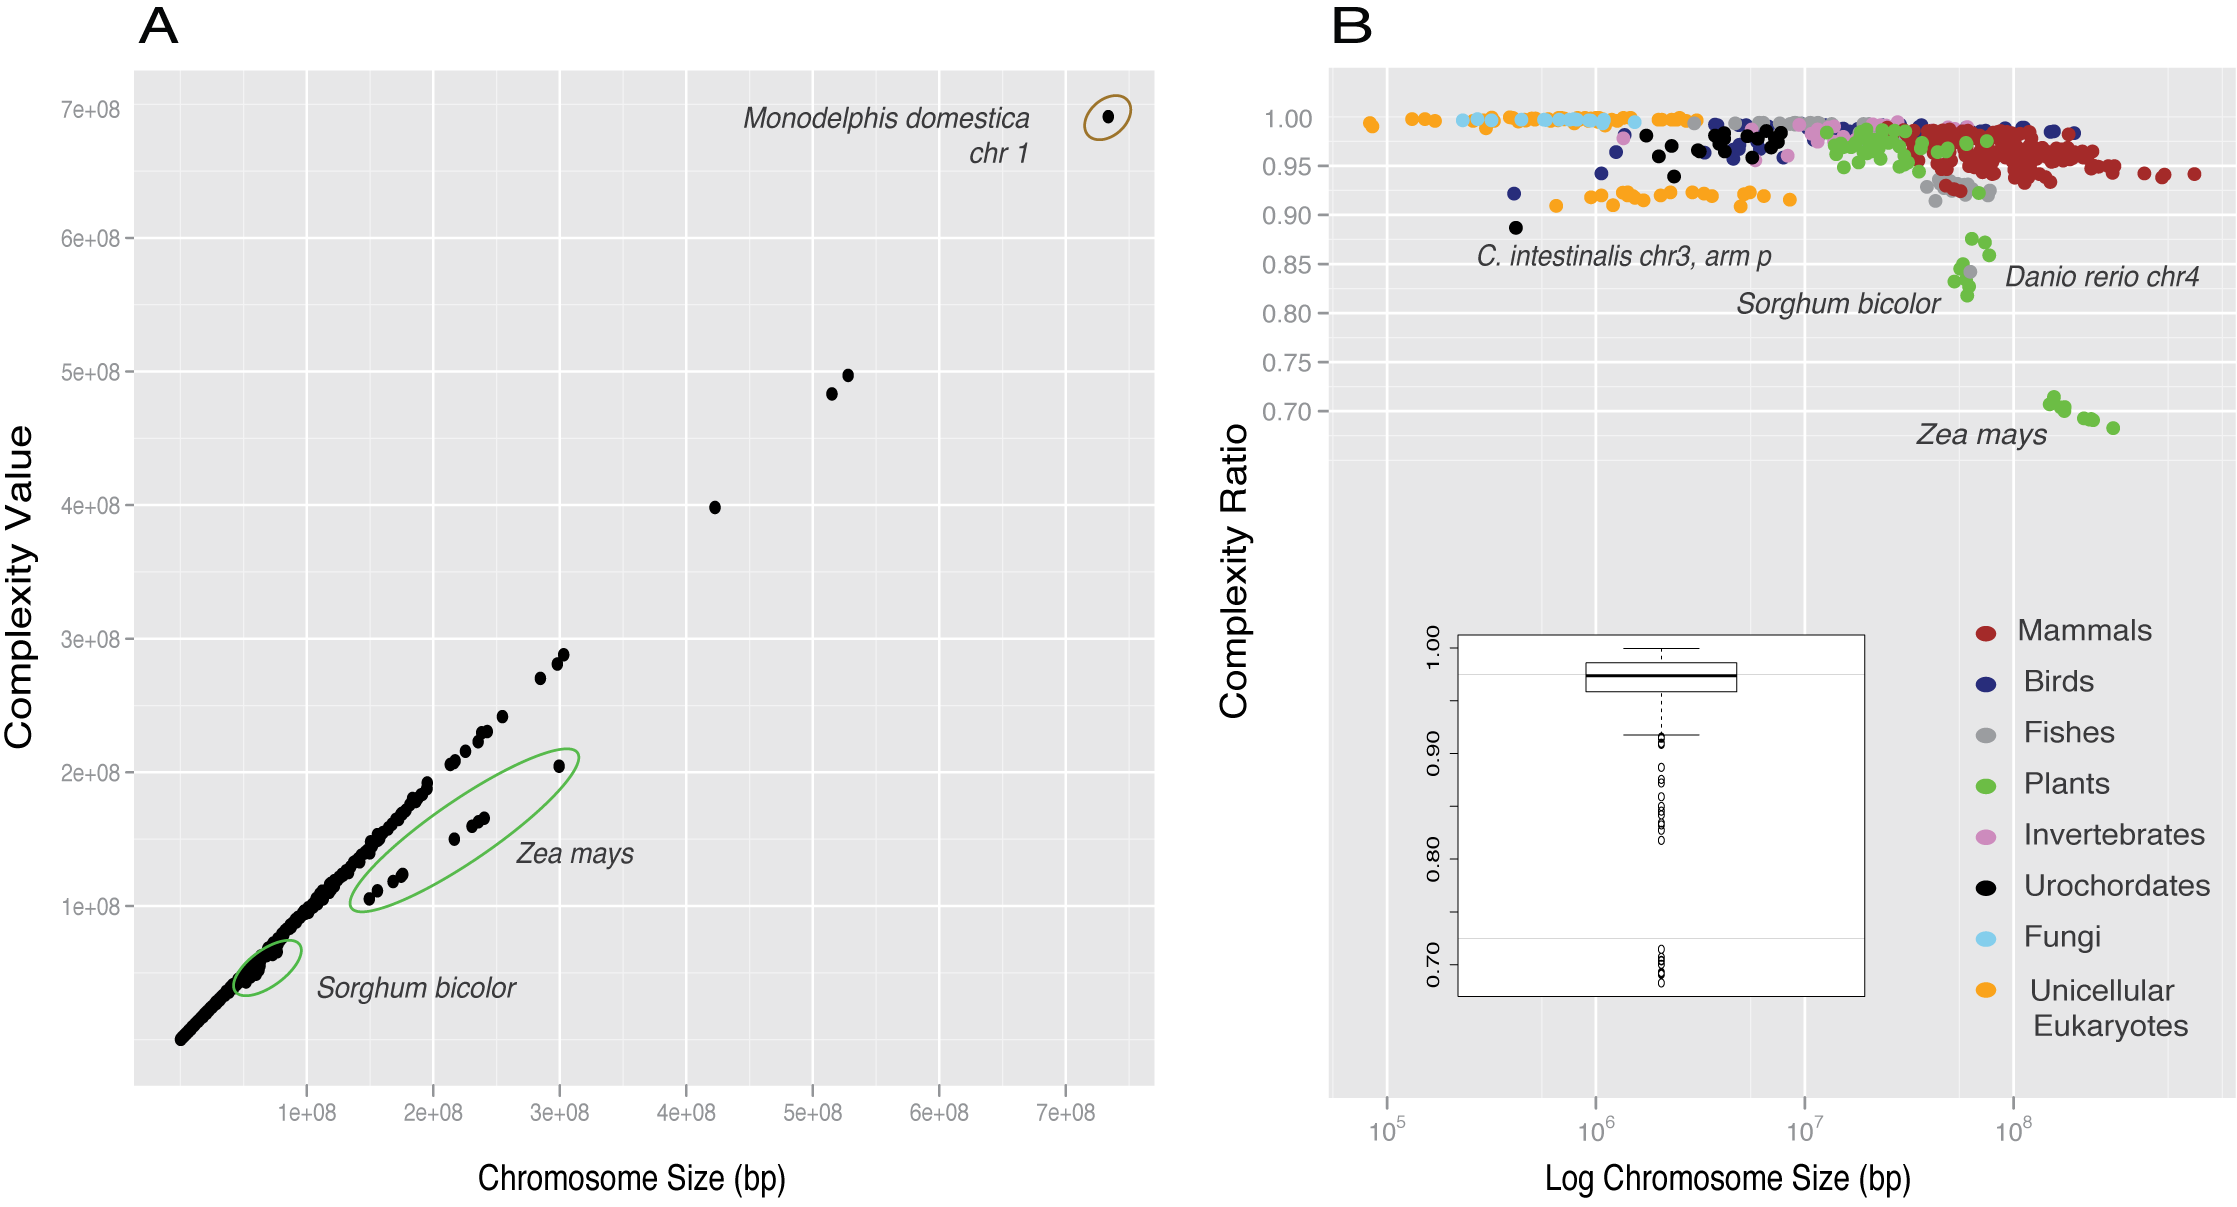
\includegraphics[width=\textwidth]{tex_source/figures/dna_struct/chromosome_complexity.png}
\caption[Chromosome complexity ratio]{{\bf Chromosome complexity ratio.} \\\textbf{(A)} Complexity ratio and chromosome size of 31 eukaryote species (567 chromosomes). Notice how far chromosomes of Z. mays, and in minor degree S. bicolor (both recent polyploid species) depart for the general trend. \textbf{(-B)} Most chromosomes (96.2\%) have complexity ratios ranging 0.9 to 1.0, as observed for complete genomes \fref{fig:gen_compl}{B}. Boxplot inside shows the distribution of CR of all
chromosomes.}
\label{fig:chr_compl}
\end{figure}

\subsection{Complexity in chromosome segments}
\label{sec:compl-chrom-segm}

Chromosomes were split in overlapping windows of various sizes (from 1 Kb to 100 Mb) and complexity ratio in these windows was computed. \fref{fig:box_compl}{} shows boxplots of six selected chromosomes, at different scales, all having extreme CR. Median values of CR over all windows of \textit{H. sapiens} Chr1 \fref{fig:box_compl}{-A}, \textit{A. thaliana} Chr1 \fref{fig:box_compl}{-C}, \textit{C. elegans} Chr1 \fref{fig:box_compl}{-D}, and \textit{D. melanogaster} Chr2L \fref{fig:box_compl}{-E} were above 0.97. Lower values were obtained in \textit{Z. mays} Chr 1 \fref{fig:box_compl}{-F} and in \textit{H sapiens} Chr19 \fref{fig:box_compl}{-B} for large windows sizes; in particular, for windows larger than 1Mb, CR noticeably fell down. The reasons for this fall are different in the two cases: while maize Chr1 is tetraploid, human Chr19 contains the highest number of Alu sequences reported in human chromosomes \cite{Venter2001}.

\begin{figure}[htpb] 
\centering 
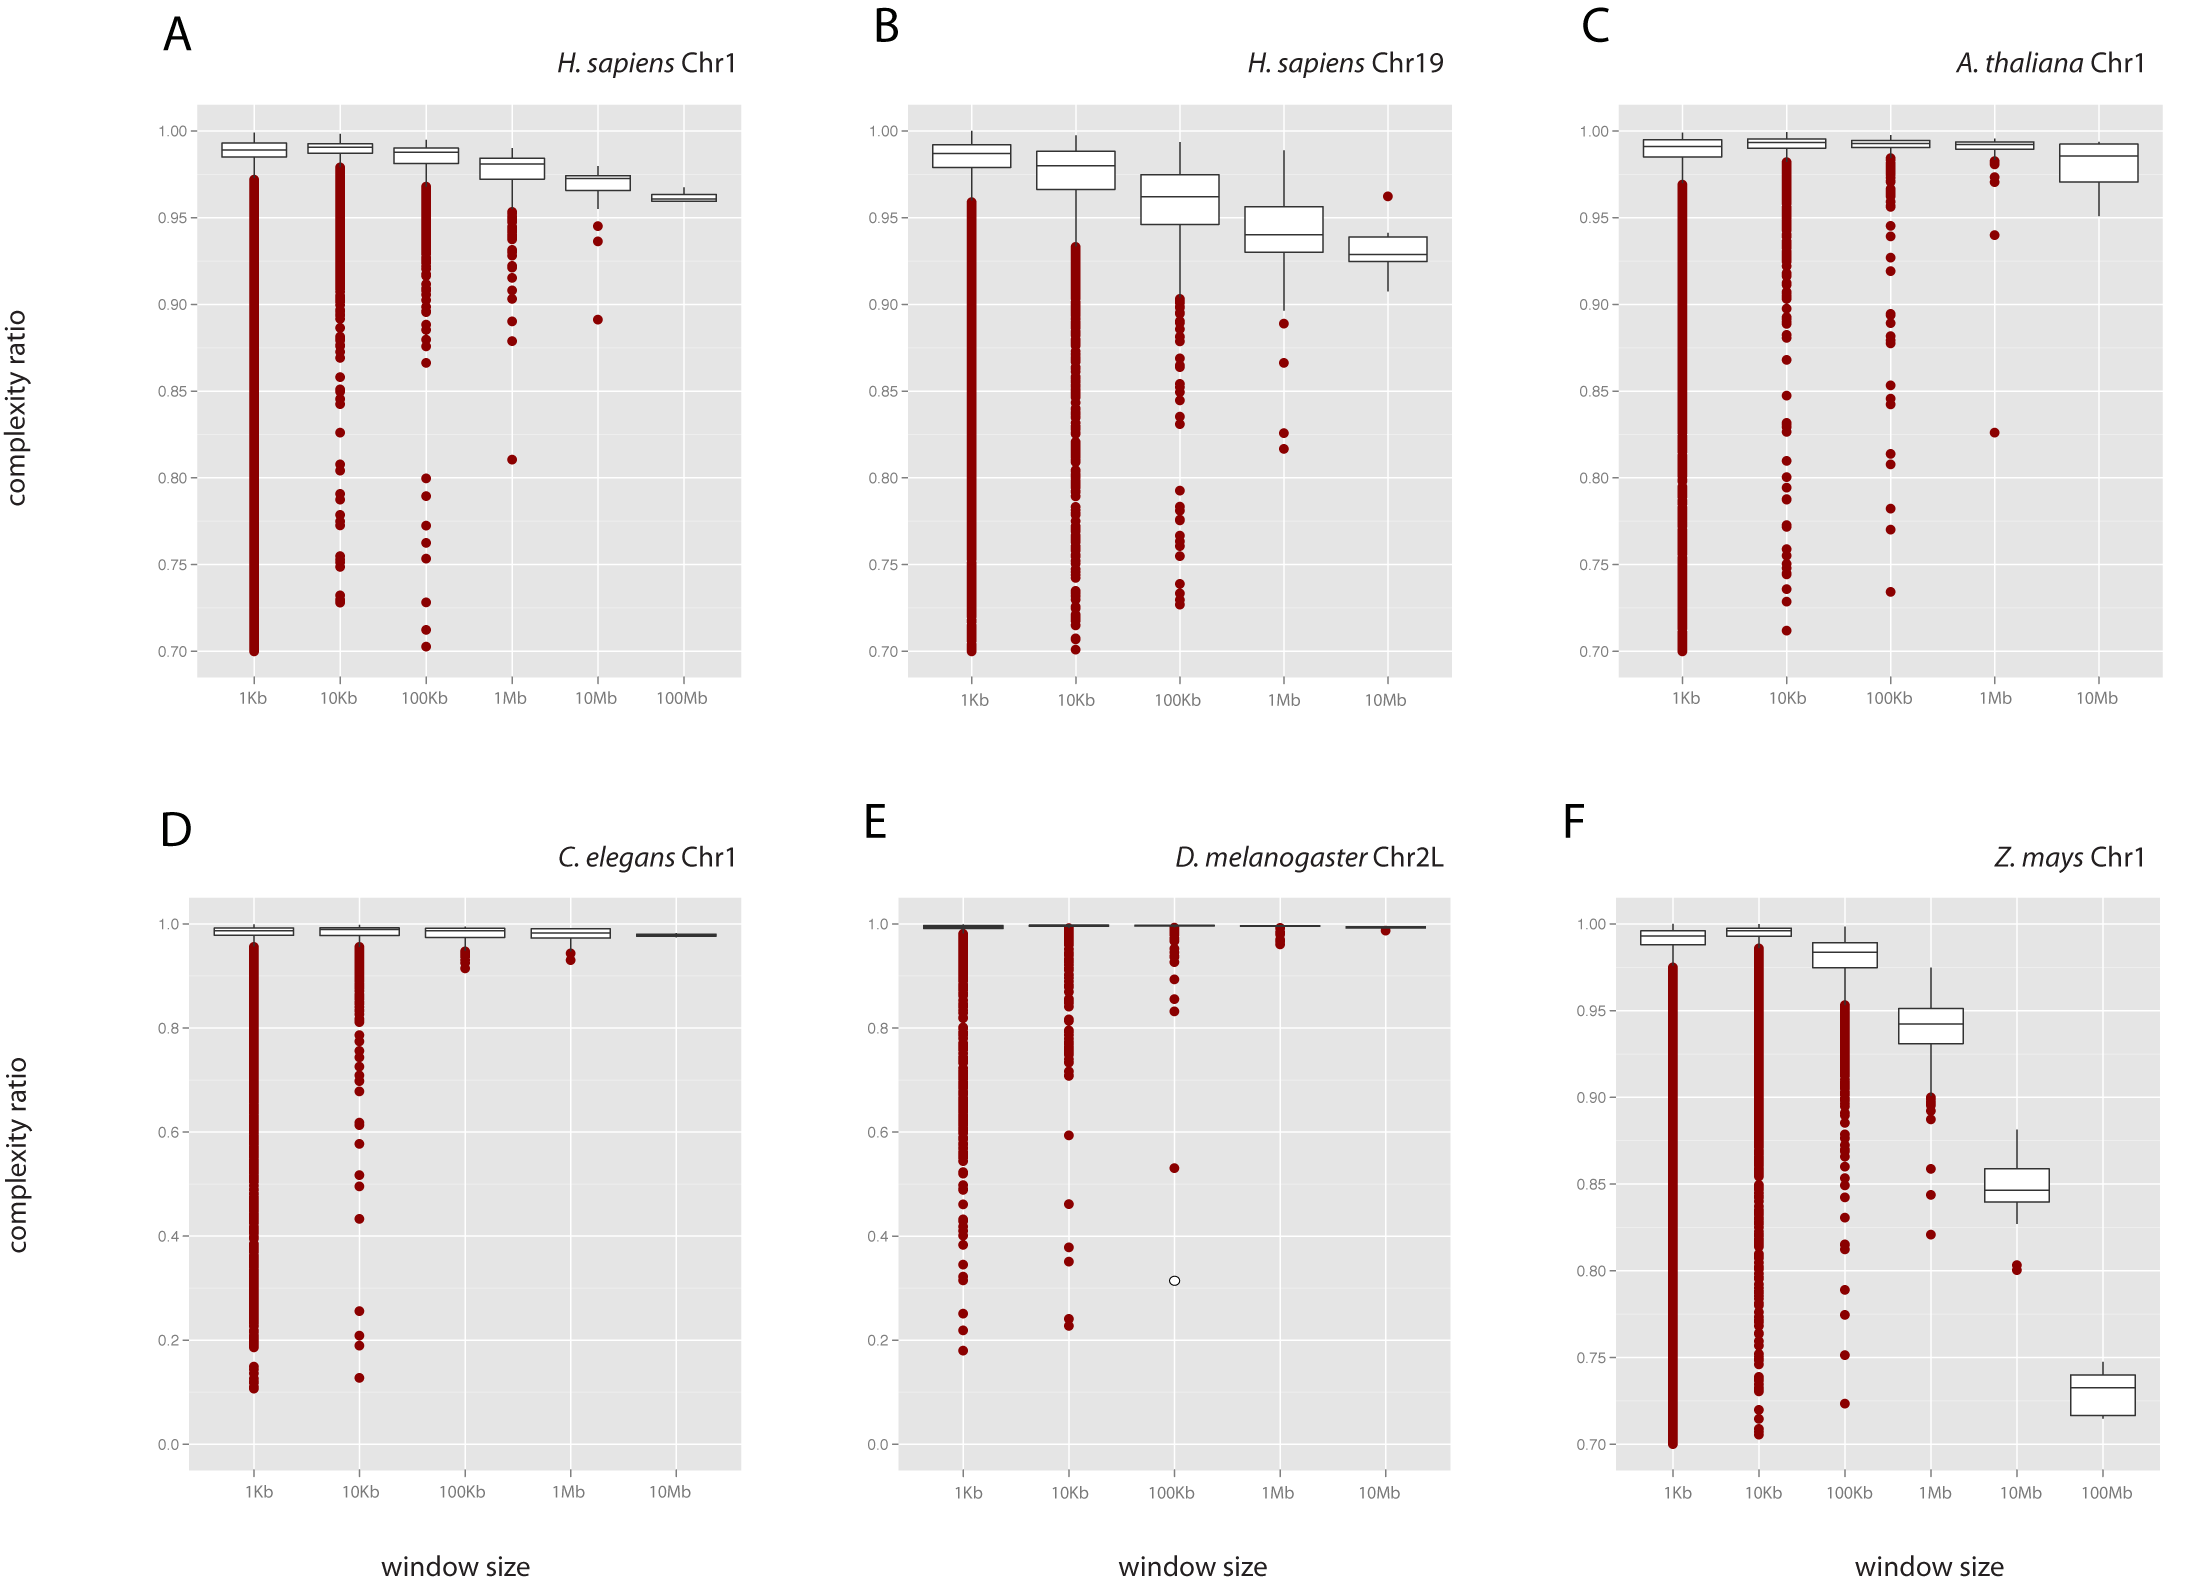
\includegraphics[width=\textwidth]{tex_source/figures/dna_struct/box_complexity_windows.png}
\caption[Sliding window analysis in chromosomes]{{\bf Sliding window analysis in chromosomes.} \\Boxplots show results of sliding window analyses in six selected chromosomes (A-F). Most chromosomes have median CR higher than 0.975 independently of window size. White dot in the 100Kb window size chart of D. melanogaster Chr 2L (E) corresponds to the ``deep spike'' displayed in \fref{fig:win_2L}{}. Scales were selected to enlarged differences in CR.
}
\label{fig:box_compl}
\end{figure}


In general, for all chromosomes, the larger the window size, the lower the median CR value. This pattern can be explained by existence of repeats, which can only be detected when the window size is large enough. In addition, CR dispersion decreases when window size increases, a fact that is explained by the substantial DNA combinatorial variation in large chromosome windows. This effect is shown in \fref{fig:win_2L}{} for window sizes of 1Kb and 100 Kb in \textit{D. melanogaster} Chr 2L, with a rugged versus smooth CR profiles. The outstanding
minimum CR ~ 0.31 was for 100 Kb-window size. This sudden decrement in CR occurred at 21,400 - 21,550 Mb where the histone cluster with more than 100 genes of the family locates.

\begin{figure}[htpb] 
\centering 
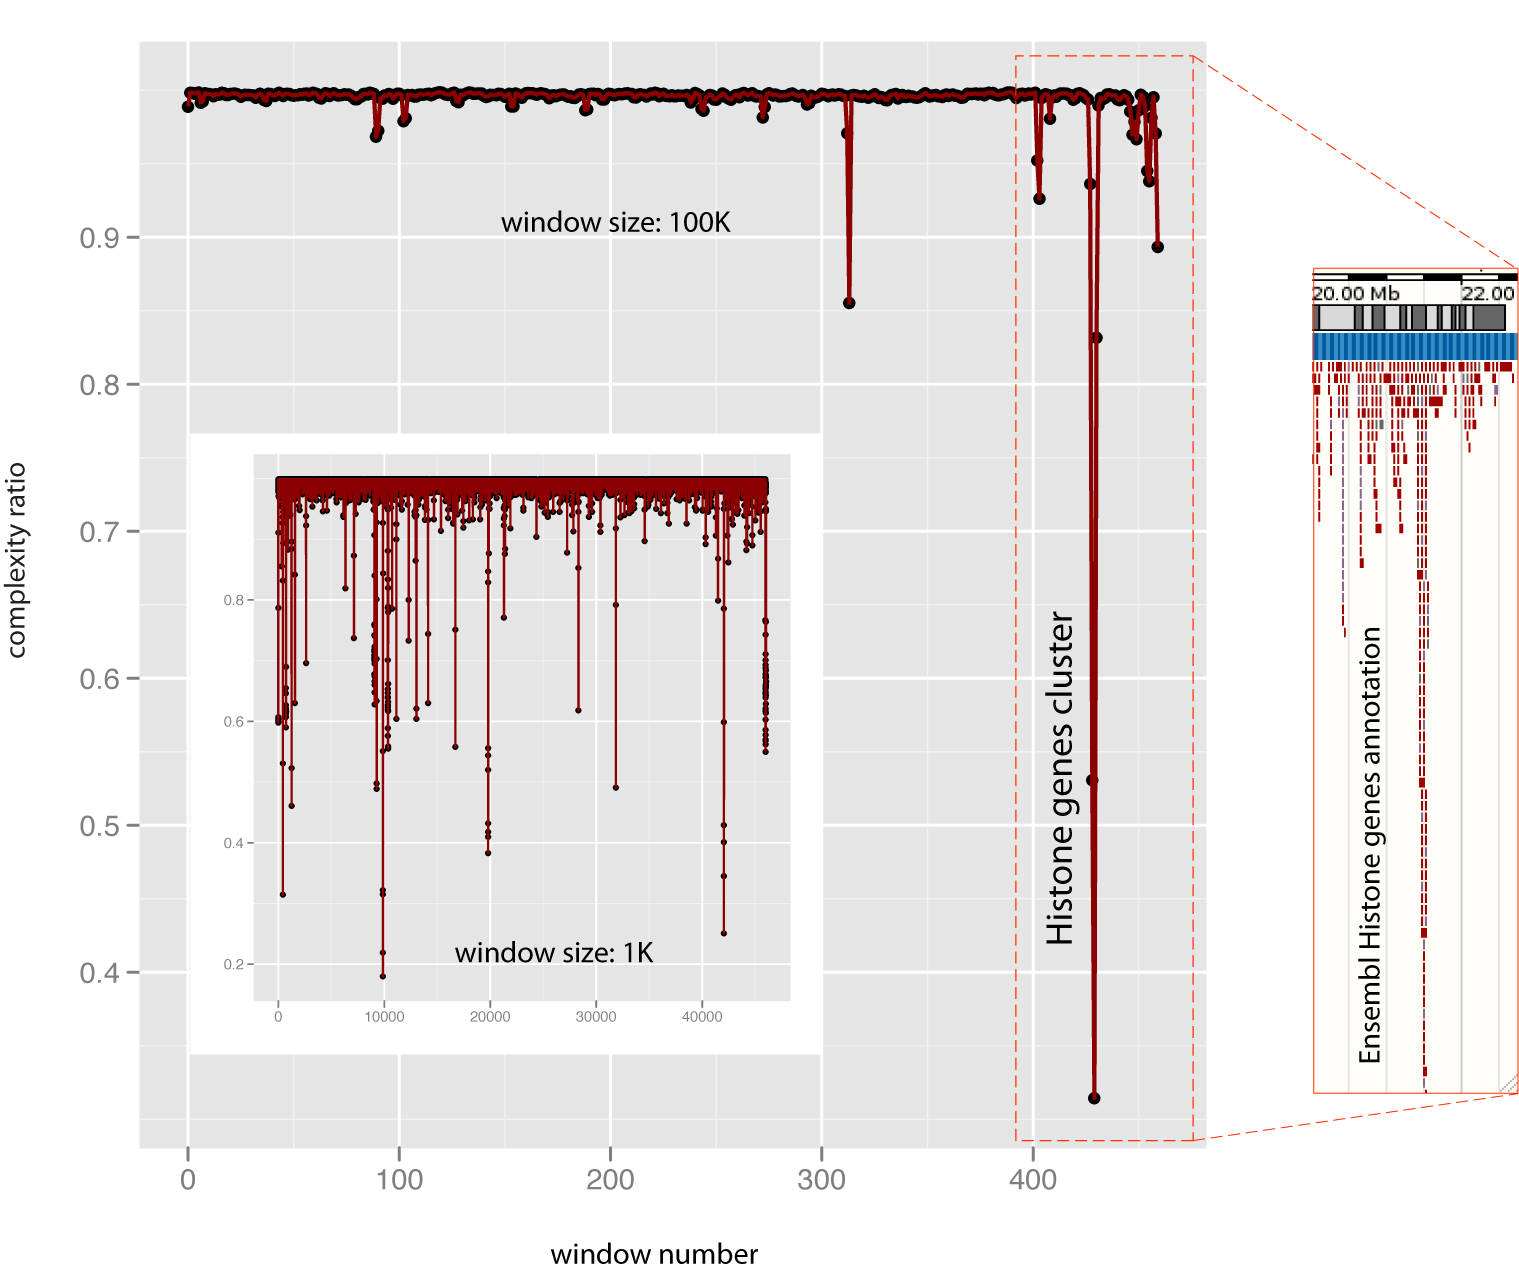
\includegraphics[width=\textwidth]{tex_source/figures/dna_struct/windows_2L.png}
\caption[Sliding window in a full chromosome]{{\bf Sliding window in a full chromosome.} \\Complexity ratio along \textit{D. melanogaster} chromosome 2L is displayed at two window size scales. Ensembl annotation of the histone genes cluster is shown in the left box. See associated DAS server displaying CR along chromosomes for 15 eukaryote species.
}
\label{fig:win_2L}
\end{figure}


The right picture shows Ensembl annotation for the histone genes cluster. The complexity values correspondind to an exhaustive sliding-window scan of chromosomes of fifteen different species is available in a DAS server at \myurl{http://bioinfo.cipf.es/das/} Complexity in repetitive elements and genes 

Eukaryote genome structure is generally sketched out by the massive presence of non-functional repetitive elements (RE-s) spread out all over the genome, and a tiny portion of singular functional elements covering the rest. To get insights into the statistical structure of these contrasting regions of genomes we computed the complexity ratio of genes and of each of the main families of RE's (as DNA-T, LTR, LINE, SINE and satellite). To do this, for each family, all units were concatenated in their original order in chromosomes, after scanning them with RepeatMasker  \cite{Smit2010} (see details of RepeatMasker output for individual species in Document S1).

Genes showed, as expected, the highest CR among all classes analyzed, independently of the species. When genes were split in their two main components, exons showed even a higher CR. Unexpectedly, high values of CR were also obtained in LINE, LTR and DNA-T (~\tref{tab:rep_compl}). In constrast, SINE and satellites showed the lowest CR. The low complexity ratio observed in SINE and satellites is mainly due to their repetitive structure, in the form of
orderly arranged short sized repetitions. The high CR associated to LINE, LTR and DNA-T (DNA-T) is explained by their larger length and their high internal variability in units of the families. In mammals DNA-T and LTR elements exhibited higher CR than LINE elements. This is not the case for fishes, some invertebrates and plants. In plants, LINE has the highest CR after genes (~\tref{tab:rep_compl} and see \fref{fig:lang_compl}{} for comparison among all eukaryote species analyzed).

\begin{table}[htbp]
\caption[Mean complexity ratio of some genome components]{Mean complexity ratio of some genome components in different species.}
\resizebox{410pt}{!}{%
  \begin{tabular}{ l r r r r r r r r }
  \hline
  \multicolumn{1}{l}{\textbf{Species}} & \multicolumn{1}{l}{\textbf{Satellite}} & \multicolumn{1}{l}{\textbf{SINE}} & \multicolumn{1}{l}{\textbf{LINE}} & \multicolumn{1}{l}{\textbf{LTR}} & \multicolumn{1}{l}{\textbf{DNA-T}} & \multicolumn{1}{l}{\textbf{Genes}} & \multicolumn{1}{l}{\textbf{Introns}} & \multicolumn{1}{l}{\textbf{Exons}} \\ \hline
  {\it H. sapiens} & 0.485 & 0.437 & 0.881 & 0.922 & 0.962 & 0.953 & 0.952 & 0.985 \\ 
  {\it P. troglodytes} & 0.491 & 0.442 & 0.885 & 0.926 & 0.962 & 0.967 & 0.965 & 0.993 \\ 
  {\it R. norvegicus} & 0.539 & 0.586 & 0.668 & 0.912 & 0.975 & 0.977 & 0.976 & 0.992 \\ 
  {\it M. musculus} & 0.595 & 0.576 & 0.74 & 0.875 & 0.973 & 0.973 & 0.97 & 0.991 \\ 
  {\it C. familiaris} & 0.6 & 0.487 & 0.911 & 0.974 & 0.982 & 0.982 & 0.98 & 0.993 \\ 
  {\it T. nigroviridis} & --- & 0.585 & 0.903 & --- & --- & 0.994 & 0.993 & 0.993 \\ 
  {\it D. rerio} & 0.628 & 0.43 & 0.796 & 0.791 & 0.824 & 0.942 & 0.936 & 0.988 \\ 
  {\it C. intestinalis} & 0.644 & 0.537 & 0.836 & 0.937 & 0.801 & 0.968 & 0.957 & 0.994 \\ 
  {\it C. elegans} & 0.52 & 0.401 & 0.93 & 0.94 & 0.827 & 0.978 & 0.957 & 0.99 \\ 
  {\it A. gambiae} & 0.232 & 0.438 & 0.805 & 0.902 & 0.771 & 0.992 & 0.992 & 0.9 \\ 
  {\it D. melanogaster} & 0.548 & --- & 0.81 & 0.744 & 0.81 & 0.985 & 0.982 & 0.99 \\ 
  {\it Z. mays} & 0.337 & 0.531 & 0.906 & 0.495 & 0.7223 & 0.962 & 0.956 & 0.975 \\ 
  {\it S. bicolor} & 0.345 & 0.619 & 0.966 & 0.602 & 0.757 & 0.99 & 0.991 & 0.988 \\ 
  {\it A. thaliana} & 0.467 & 0.675 & 0.971 & 0.84 & 0.896 & 0.989 & 0.986 & 0.988 \\ 
  {\it A. lyrata} & 0.417 & 0.457 & 0.928 & 0.772 & 0.826 & 0.994 & 0.988 & 0.996 \\ \hline
  \end{tabular}
}
\label{tab:rep_compl}
\end{table}


For each family, we used the complexity ratio to describe the disposition of the elements inside a chromosome. CR of linearly arranged elements was compared to the CR of shuffled elements. \tref{tab:compl_rep} shows these values for eight selected chromosomes of different species. CR in the linear arrangement was much lower in SINE and satellites than in the rest of the classes. This reveals a structure of identical or very similar repeats along neighbor chromosome segments. This pattern did not showed up in the other families. The notable exception was LTR of the maize chromosome, known to have expanded dramatically in recent evolutionary times \cite{Blanc2004}. All shuffled classes (including SINE and satellites) had a CR equal to one, or very close to one. This entails an almost uniform statistical distribution of DNA sequences in that class. This result point outs that genomes are plenty of genetic variation, even in regions where the expected pattern is the homogeneous repetition of almost indistinguishable units of RE's.

\rowcolors{1}{white}{white}
\begin{table}[htbp]
\caption[Complexity ratio of genome classes concatenated and shuffled]{Size and complexity ratio of different genome classes concatenated (CON), and shuffled (SHU) for selected chromosomes. Size in Mb.}
\resizebox{410pt}{!}{%
  \begin{tabular}{ l l r r r r r r r r }
  \hline
   &  & \multicolumn{ 2}{c}{\textbf{\em A. thaliana}} & \multicolumn{ 2}{c}{\textbf{\em C. elegans}} & \multicolumn{ 2}{c}{\textbf{\em H. sapiens}} & \multicolumn{ 2}{c}{\textbf{\em Z. mays}} \\ \hline
   &  & Chr 1 & Chr 5 & Chr 1 & Chr 2 & Chr 1 & Chr 21 & Chr 1 & Chr 10 \\ \hline
  \multicolumn{ 1}{c}{} & SIZE & 0.476 & 0.147 & 0.159 & 0.149 & 0.172 & 0.118 & 0.48 & 0.288 \\
  \multicolumn{ 1}{c}{Satellite} & CON & 0.223 & 0.299 & 0.489 & 0.547 & 0.519 & 0.567 & 0.325 & 0.309 \\ 
  \multicolumn{ 1}{l}{} & SHU & 0.889 & 0.968 & 0.962 & 0.975 & 0.972 & 0.987 & 0.961 & 0.948 \\ \hline
  \multicolumn{ 1}{c}{} & SIZE & 0.023 & 0.023 & 0.009 & 0.007 & 35.782 & 3.979 & 0.051 & 0.023 \\ 
  \multicolumn{ 1}{c}{SINE} & CON & 0.69 & 0.682 & 0.367 & 0.402 & 0.439 & 0.433 & 0.525 & 0.531 \\ 
  \multicolumn{ 1}{l}{} & SHU & 0.976 & 0.975 & 0.956 & 0.943 & 0.925 & 0.942 & 0.945 & 0.951 \\ \hline
  \multicolumn{ 1}{c}{} & SIZE & 0.121 & 0.146 & 0.039 & 0.026 & 26.321 & 3.778 & 1.454 & 0.739 \\ 
  \multicolumn{ 1}{c}{LINE} & CON & 0.975 & 0.972 & 0.93 & 0.982 & 0.874 & 0.905 & 0.899 & 0.916 \\ 
  \multicolumn{ 1}{l}{} & SHU & 1.000 & 1.000 & 0.999 & 1.000 & 0.999 & 1.000 & 1.000 & 1.000 \\ \hline
  \multicolumn{ 1}{c}{} & SIZE & 0.914 & 0.944 & 0.022 & 0.013 & 10.474 & 2.11 & 115.466 & 57.56 \\ 
  \multicolumn{ 1}{c}{LTR} & CON & 0.811 & 0.809 & 0.98 & 0.984 & 0.906 & 0.93 & 0.47 & 0.513 \\ 
  \multicolumn{ 1}{l}{} & SHU & 0.998 & 0.998 & 1.000 & 1.000 & 0.999 & 1.000 & 0.993 & 0.995 \\ \hline
  \multicolumn{ 1}{c}{} & SIZE & 0.68 & 0.541 & 0.704 & 0.518 & 3.734 & 0.552 & 6.066 & 3.109 \\ 
  \multicolumn{ 1}{c}{DNA-T} & CON & 0.883 & 0.887 & 0.81 & 0.84 & 0.95 & 0.98 & 0.7 & 0.74 \\ 
  \multicolumn{ 1}{l}{} & SHU & 0.999 & 0.999 & 1.000 & 1.000 & 1.000 & 1.000 & 1.000 & 1.000 \\ \hline
  \multicolumn{ 1}{c}{} & SIZE & 18.242 & 16.312 & 10.77 & 9.918 & 140.258 & 21.909 & 37.623 & 16.759 \\ 
  \multicolumn{ 1}{c}{GENES} & CON & 0.988 & 0.989 & 0.975 & 0.981 & 0.951 & 0.964 & 0.956 & 0.967 \\ 
  \multicolumn{ 1}{l}{} & SHU & 1.000 & 1.000 & 1.000 & 1.000 & 1.000 & 1.000 & 1.000 & 1.000 \\ \hline
  \multicolumn{ 1}{c}{} & SIZE & 5.318 & 4.73 & 6.074 & 4.94 & 130.429 & 20.696 & 22.229 & 9.735 \\ 
  \multicolumn{ 1}{l}{INTRON} & CON & 0.985 & 0.986 & 0.95 & 0.963 & 0.95 & 0.964 & 0.948 & 0.966 \\ 
  \multicolumn{ 1}{l}{} & SHU & 1.000 & 1.000 & 1.000 & 1.000 & 1.000 & 1.000 & 1.000 & 1.000 \\ \hline
  \multicolumn{ 1}{c}{} & SIZE & 12.925 & 11.582 & 4.694 & 4.979 & 9.829 & 1.213 & 15.394 & 7.024 \\ 
  \multicolumn{ 1}{c}{EXON} & CON & 0.988 & 0.989 & 0.991 & 0.991 & 0.983 & 0.99 & 0.972 & 0.976 \\ 
  \multicolumn{ 1}{l}{} & SHU & 1.000 & 1.000 & 1.000 & 1.000 & 1.000 & 1.000 & 1.000 & 1.000 \\ \hline
  \end{tabular}
}
\label{tab:compl_rep}
\end{table}


Polyploidy and return to maximum complexity Evolution erodes ancient footprints of genome polyploidy and diploidization (the process by which a polyploid genome turns into a diploid one) proceeds during time \cite{Wolfe2001}. As shown in previous sections, CR of recent polyploids is much lower than in non-polyploid, or in ancient polyploid species. Diploidization can be achieved by multiple mechanisms \cite{Wolfe2001}, being the gradual disintegration of the duplicated genetic material by random mutation. This is the simplest form. However, more dramatic mechanisms such as massive deletion, and transpositions of genetic material was reported in \textit{A. thaliana} \cite{Hu2011}. We tested the hypothesis that the complexity ratio of polyploid genomes increases along the diploidization process.

Polyploid origin and posterior decay of genetic redundancy was simulated by means of mutations and transpositions in random sequences of different lengths and ploidy levels, and in \textit{Z. mays} Chr1 and \textit{S. bicolor} Chr1 (Figure 5). In all cases, sequences under random mutation and transposition reached maximum CR=1 after a number of generations large enough. Larger sequences representing genomes or chromosomes increased their CR faster than shorter sequences. This is as expected in probability theory since each sigle choice (introduced by a random mutation or a transposition) in a large set is more informative than in a smaller set, because it makes a selection in a bigger space of possibilities. The dynamics of CR increase was identical for the maize and sorghum chromosomes and the simulated random sequences (Figure 5A). Figure 5B shows that genomes and chromosomes reached maximum CR=1 after many cycles of transpositions. Using a simulated genome with tetraploid structure, transposition preserved the relation that chromosome CR is higher than genome CR, along all generations up to convergence to maximum CR=1. This feature was reported above for maize and sorghum (see discussion on chromosome complexity ratio).

Once CR reached almost maximum complexity any signal of polyploidy is finally lost, and DNA structure is indistinguishable from diploid genomes. High complexity and random-like structure of DNA Excluding recent polyploids, high CR (almost maximum) was observed in complete genomes of organisms sampled in all diversity of life, in their chromosomes and along large enough chromosomes segments, and in shuffled arrangements of elements in individual genetic classes. We conjecture this is a universal feature of all genomic sequences. Polyploids were the only DNA sequences on which we obtained low complexity ratios, hence, they are the only DNA sequences with the distinguishing feature low CR: Low CR corresponds to a simple combinatorial structure of the sequence. 

The combinatorial structure of a sequence is a description of the observed arrangement of the symbols among all possible permutations of the same length. Sequences with many long repeats have low CR. Sequences with the minimum CR=0 consist of a single symbol (as $AAAAAAAAAA$) -this is the simplest combinatorial structure- so they are plainly compressible. Polyploid genomes of maize and sorghum have CR=0.585, and CR=0.786, respectively. Values that were close to the simulated tetraploid genomes (Fig 5B). It is also possible to achieve low CR in sequences without any long repeats, but with an orderly arrangement of the symbols. Although we have not found this phenomena in natural DNA, we constructed de Bruijn sequences (these are the mathematically defined sequences with perfect equifrequency of subsequences: every possible sequence of logarithmic length appears exactly once as a sequence of consecutive symbols) \cite{DeBruijn1946,Becher2011} with low CR. The regularity in the combinatorial structure of these particular de Bruijn sequences is captured by the MTF algorithm. See Appendix I for examples on short sequences. High complexity ratio implies the following properties on the combinatorial structure of DNA sequences: High CR corresponds to high diversity and balanced abundance of short repeats. Maximum CR=1 is reached by sequences a sequence of length n if it contains full diversity of length k, for k ! log4 n, and each these short sequences occur about n*4-k times. As CR decreases, diversity and balanced abundance deteriorates. In particular, maximum CR is holds for some de Bruijn sequences \cite{DeBruijn1946,Becher2011}. Also maximum CR=1 occurs in randomly generated sequences with uniform distribution of A, C, G, T. For genomic sequences \cite{Liu2008} reported that more than 98\% of 12 bp oligomers appear in vertebrate genomes while less than 2\% of 19 bp oligomers are present. For the human genome we computed all maximal exact repeats over 30 bp, and counted their diversity and quantity \cite{Nies2009}. We observed that the largest correlations in the human genome are intrachromosomal, the actual largest exact repeat is 67,632bp long and it occurs just twice inside Chr 1, while the largest inter-chromosomal perfect correlation is 21,865 bp occurring just once Chr 1 and once in Chr 5.

High CR corresponds to random-like sequences. Intuitively, a non random sequence will exhibit some significant regularity that can be used to compress the sequence. The mathematical underpinning relies on the theory of pure randomness \cite{Chaitin1975,Nies2009}, which states that an infinite sequence is random when its initial segments are incompressible. Up to some deviations, for finite sequences and particular compression methods, the identification between statistical randomness and incompressibility holds. The complexity ratio (CR) expresses incompressibility by the BWT-MTF scheme and further encoding as determined by Shannon's entropy. High complexity ratios correspond to highly incompressible sequences, which are sequences with a random-like structure. As in statistical randomness, the number of sequences with high CR grows exponentially with the sequence length. Thus, each genome is a singular instance out of the extraordinary many combinatorial variants of the same length with the same high complexity rate. A lower bound of the number of sequences with high CR (CR `` 1 - !, for any real value ! between 0 and 1) is proved Appendix II.


\section{Material and methods}
\label{sec:dna_struct-matmet}

\subsection{The complexity ratio and complexity value}
\label{sec:compl-ratio-compl}

Complexity Ratio (CR) is defined by a classical formula used in data compression \cite{Adjeroh2008}, the Burros-Wheeler transform BWT \cite{Burrows1994}, followed by the Move To Front (MTF) \cite{Ryabko1980} and finally resume this to one value using Shannon's entropy \cite{Shannon1948}. Thus the CR is Shannon's entropy of a transformation or digestion of the sequence. The purpose of this transformation is to reveal the regularities in a sequence. In case the original sequence has no significant regularities, all numbers will be at the same rate; else, some numbers will be in excess and others in shortage (compression algorithms use this to obtain a short output). Shannon's entropy is zero -this is the minimum- only when all numbers are zero. This occurs when a sequence consists just of a single repeated symbol, which is the simplest possible combinatorial structure. When, at the other edge, entropy is equal to one (the maximum entropy), then all numbers have exactly the same frequency, and it indicates that the sequence has a random-like combinatorial structure. 
Algorithmically, the BWT of a given sequence is a permutation of the symbols in the sequence that represents the lexicographic order of all possible rotations of the sequence. The MTF transforms a given sequence into a sequence of numbers, operating from left to right, and maintaining a stack of recently used symbols. Each number is an index in the stack and denotes an alphabet symbol. Shannon's entropy maps a sequence into a real number between zero and one. It weights the frequency of the alphabet symbols in a given sequence. For each symbol $i$ in the alphabet, let $p_{(i)}$ be the probability of finding $i$ in the sequence $s$; $N_i$ the number occurrences of $i$ in $s$ and $length(s)$ the total length of the sequence $s$: 

\begin{equation} \label{eq:prob_seq}
p_{(i)} = \frac {N_i}{length(s)}
\end{equation}

For DNA alphabet entropy is defined as:

\begin{equation} \label{eq:entropy}
E(s) = -\sum_{i=0}^{\exists}p_{(i)} \times log_4(p_{(i)})
\end{equation}

Thus the CR can be factorize as:

\begin{equation} \label{eq:cr}
CR(s) = E(MTF(BWT(s)))
\end{equation}

The complexity value (CV) of a sequence is its CR times the number of
characters in this sequence (here $s$):

\begin{equation} \label{eq:cv}
CV(s) = E(MTF(BWT(s))) \times length(s)
\end{equation}

As the CV of a sequence depends on the transformation of the MTF applied to the whole sequence, its computation impede the use of parts of the sequence independently.

\subsection{Complexity in strings}
\label{sec:complexity-strings}

Complete genomes of 54 species were download from NCBI and Ensembl Genome Project \cite{Flicek2011}. Fourteen major groups of taxa were selected: virus, phages, bacteria, archaea, fungi, amplicomplexa, heterokonta, amebozoa, urochordates, invertebrates, plants, fishes, birds, and mammals. Species among taxa were chosen to the interest as model species and the presence of particular biological features such as: variation in genome size, ancestral and recent polyploidy, living in extreme environments, living as intracellular parasites, gene expansion, genome reduction, RNA or single-strand DNA genomes, and synthetic genomes \tref{tab:genome}. Eukaryote genomes with coverage of 6$\times$ or greater were chosen. Sexual chromosomes were excluded from the analysis, and ambiguous ``N'' characters were removed from sequences, and not taken into account when computing chromosome length. Eukaryote chromosomes were concatenated in genomes to estimate genome complexity. Interspersed repeats and low complexity DNA sequences were screened and mapped in chromosomes of thirty different eukaryotes using RepeatMasker \cite{Smit2010}. Complexity of major families of repetitive elements such as DNA transposons, LTR, LINE, SINE, satellites and exons, introns, and complete genes (considering unstranslated regions) was computed after concatenation of all elements in chromosomes excluding. Random sequences with different ploidy levels were generated in python. Complexity value of biological sequences and random sequences was computed with the DNA alphabet of four letters. Complexity in biological sequences was computed in the +1 strand. Analyses of -1 strand provided no differences in results. Short stories, books and complete works in its original languages were downloaded from Project Gutember (\myurl{http://www.gutenberg.org/}). To automatically detect the alphabet size in texts (including mathematical and punctuation symbols) we run COMPL program with ``auto'' option. To study complexity along chromosomes, a sliding window method shifting along chromosomes in overlapping units of 1.0 Kb to 100 Mb was performed. Linear models, and linear models with interactions were run in R language \cite{Team2008}.

\subsection{Simulations}

We performed four kinds of experiments where complexity value and ratio were computed. First: random polyploid construction of sequences of various sizes and ploidy levels (one to ten). Second: the evolution along 40 million generations by constant neutral mutation rate of 1.0e-08 mutations per site per generation (this value is in between the mutation rate estimated for {\it Homo sapiens}: 2.5e-08 \cite{Nachman2000} , and \textit{Arabidopsis thaliana}: 7.1e-09 \cite{Ossowski2010}) on random sequence, and on chromosomes of \textit{Zea mays} and \textit{Sorghum bicolor}. Third: the evolution along 50,000 generations of random polyploid genomes of different sizes (100Kb, 1Mb, 10Mb) by transpositions of a fixed length (1.0 Kb) between chromosomes. The number of transposition per generation was set as a constant function of genome size (genome size/1,000). Last: the concatenation and shuffling (computed with the python base function: ``shuffle'') of all repetition instances in chromosomes for main repetitive families, and genes were considered. Complexity value and ratio were computed every 100 generations. 

\section{Discussion}

However it is striking that whatever subgroup of elements we selected (\textit{Simple repeats}, \textit{Satellites}...), no perfect random structure was found in any of the steps of life complexity. Sequences can be divided into modules of nucleotides as mentioned in \cite{Wagner2007} or defined by Herzel and collaborators \cite{Herzel1995} when it fulfill 3 requirements, concisely:
\begin{itemize}
\item \textbf{Requirement 1}: must occur more frequently than expectation by random.
\item \textbf{Requirement 2}: must not be included into a larger module.
\item \textbf{Requirement 3}: must be non-overlapping between them.
\end{itemize}

%%% Local Variables: 
%%% mode: latex
%%% TeX-master: "../../master"
%%% End: 
